\documentclass[a4paper,12pt,headsepline]{scrartcl}
\usepackage{amssymb}
\setcounter{tocdepth}{3}
%\setcounter{secnumdepth}{-2}
\usepackage{graphicx}
\usepackage{rotating}
\usepackage{float}
\usepackage{url}
\usepackage{hyperref}
\usepackage[ngerman,nameinlink]{cleveref}
\usepackage{array}
\usepackage{longtable}
\usepackage{listings}
\usepackage{color}
\usepackage{transparent}
\graphicspath{{Images/}}
\usepackage[utf8]{inputenc}
\usepackage{setspace}
\usepackage[ngerman]{babel}



\begin{document}
	
	\begin{verbatim}
	
	
	\end{verbatim}
	
	\begin{center}
		\Large{Universität Kassel}\\
		\Large{Fachbereich 16 - Informatik und Elektrotechnik}\\
	\end{center}
	
	
	\begin{verbatim}
	
	
	
	
	\end{verbatim}
	\begin{center}
		\doublespacing
		\textbf{\LARGE{Teamarbeit}}\\
		\singlespacing
		\begin{verbatim}
		
		\end{verbatim}
		\textbf{Abschlussbericht}
	\end{center}
	\begin{verbatim}
	
	\end{verbatim}
	\begin{center}
		
	\end{center}
	\begin{verbatim}
	
	\end{verbatim}
	\begin{center}
		
	\end{center}
	\begin{verbatim}
	
	
	
	
	\end{verbatim}
	\begin{flushleft}
		\begin{tabular}{llll}
			\textbf{Autoren:} & & Dennis Knitterscheidt & \\
			& & Robert Meschkat & 28227496\\
			& & Philipp Schenk & 33309370\\
			& & Eric Wagner & 32233447\\ \\
			\textbf{Betreuer:} & & M. Sc. Stephan Opfer &\\
		\end{tabular}
	\end{flushleft}
	\newpage
	
	\tableofcontents
	\newpage
	
	\section{Einleitung}
		Philipp\\
		REMOVE THIS: \href{https://docs.google.com/document/d/1wGlFley6lwhnpLsj8ms7M6fnOjplazlHNr8Bfbv3vso/edit}{Beispiel}\\\\
		Kurze Beschreibung des Themas Teamarbeit. Was ist der Bericht?
	\newpage
	\section{Technische Arbeit}
	
	\subsection{Arbeitsauftrag}
Im KickOff-Workshop zur Veranstaltung \glqq Teamarbeit\grqq\ wurden mehrere Aufgaben vorgestellt. Das Team hat sich dann zusammen gefunden, um folgende Aufgabe zu bearbeiten: \\
Für die vom Team bearbeitete Aufgabe sollten ein Turtlebot und die existierende Software so erweitert werden, dass der Turtlebot als Transportsystem im Fachgebiet eingesetzt werden kann. Der Turtlebot sollte über die Software an einen Ort im Fachgebiet geschickt werden können, an dem er einen Gegenstand entgegen nimmt. Der Gegenstand sollte dann an einen vorher in der Software definierten Zielort gebracht werden. \\
Für die Umsetzung sollte ein Behältnis  für den Transport der Gegenstände auf dem Turtlebot befestigt werden. Der Behälter sollte mit entsprechender Sensorik ausgestattet werden, damit der Turtlebot erkennt, wenn ein Gegenstand auf ihm plaziert wurde. Da der Turtlebot nur Daten verarbeiten kann, die sich in seinem Weltmodel befinden, mussten die Sensordaten außerdem in das bestehende Framework eingepflegt werden.\\
Um dem Turtlebot den Transportauftrag zu erteilen, sollte eine graphische Benutzeroberfläche entwickelt werden, in der man den Start- und Zielpunkt, sowie den zu transportierenden Gegenstand festlegen können soll.  

		
%\begin{itemize}
%\item Erstellen eines Transporters aus einem Turtlebot
%\item Anbindung eines Drucksensors unter einen Tragekorb
%\item Integration der Sensorwerte in das bestehende Framework
%\item UI zum Steuern entwickeln
%\item Testen und Evaluieren
%\end{itemize}
	
\subsection{Entwurft}
\subsubsection{Erste Bestandsaufnahme}
Da kein Teammitglied zuvor mit den Turtlebots gearbeitet hat, musste sich das Team zunächst einen groben Überblick über die bestehende Hard- und Software verfassen, bevor mit der eigentlichen Planung begonnen werden konnte.\\
Für die Sensorik des Behälters war der Aufbau des Turtlebots ausschlaggebend: Gesteuert wird der Turtlebot von einem Notebook. Dieses ist über USB sowohl mit der Fahrbasis, als auch mit der Sensorik für die räumliche Erkennung verbunden. Damit wurde klar, dass auch der Gegenstandsdetektor über USB mit dem Notebook verbunden werden muss. \\
Die Software-Sammlung, die für den Betrieb des Turtlebots benötigt wird, basiert auf dem \glqq Robot Operating System\grqq , kurz ROS genannt, in der Version \textit{Kinetic} und ist in C++ verfasst. Das User Interface musste als mit ROS kommunizieren können und im besten Fall in C++ geschrieben sein.

\subsubsection{Recherche}
Nachdem die Rahmenbedingungen abgeklärt waren, begann das Team zunächst mit der Suche nach Lösungen für die Aufgabenstellung.\\
Bei der Sensorik für die Gegenstandserkennung hat sich das Team schnell auf einen Taster festgelegt, der ausgelöst werden soll, wenn ein Objekt in den Behälter gelegt wird. Kurzzeitig war auch noch ein RFID-Leser im Gespräch, der zusätzlich oder anstelle des Taster angebracht werden sollte. Mit dem Lesegerät hätten zwar die zu transportierenden Gegegenstände identifiziert werden können, allerdings hätten dann auch alle Objekte mit einem entsprechenden Marker versehen werden müssen. Daher entschied sich das Team für den Taster, der beim Transport den größeren Spielraum lässt und außerdem leichter umzusetzen war. \\
Für die mögliche Umsetztung des Tasters gab es verschiedene Lösungsansätze: Die einfachste Lösung wäre ein bereits fertiger Taster mit USB-Anschluss, der zum Beispiel eine Tastaturtaste simuliert. Die Recherche des Teams zeigte, dass entsprechende \glqq Ein-Knopf-Tastaturen\grqq\ tatsächlich existieren, sich jedoch preislich in keinem realistischem Rahmen bewegen. Ein weiterer Vorschlag war die Modifikation eines Peripheriegerätes, wie Maus oder Tastatur. Auch diese Idee wurde verworfen, da sie vom Team als zu aufwändig und als mögliche Fehlerquelle angesehen wurde. \\
Für die Entwicklung des User Interfaces wurden zwei C++-Bibliotheken evaluiert: Zum einen der Quasi-Standard \glqq Qt\grqq\ und zum anderen das \glqq Chromium Embedded Framework\grqq , kurz CEF. Bei der Evaulation stellte sich das CEF als interresante Lösung heraus, wurde aber vom Team aber abgelehnt, da es für dieses Projekt als zu aufwändig erschien. \\
Als Plattform für die Entwicklung wollte das Team sowohl das im Fachgebiet eingesetzte Ubuntu 16.04 LTS mit ROS Kinetic, als auch das zu diesem Zeitpunkt aktuelle Ubuntu 18.04 LTS mit ROS Melodic erproben.

\subsubsection{Erster Entwurf}	
Nach der Recherche entschied sich das Team dazu den Taster selbst zu bauen. Dafür sollte er mit einem Microcontroller verbunden werden, der die Signale über USB an das Notbook überträgt. Als Microcontroller wurde der \glqq Digispark Rev. 3\grqq\ (\cref{fig:digispark}) gewählt, da er mit seinen kleinen Abmessungen und seinem geringen Preis eine gute Lösung zu sein schien. 

\begin{figure}[H]
\centering
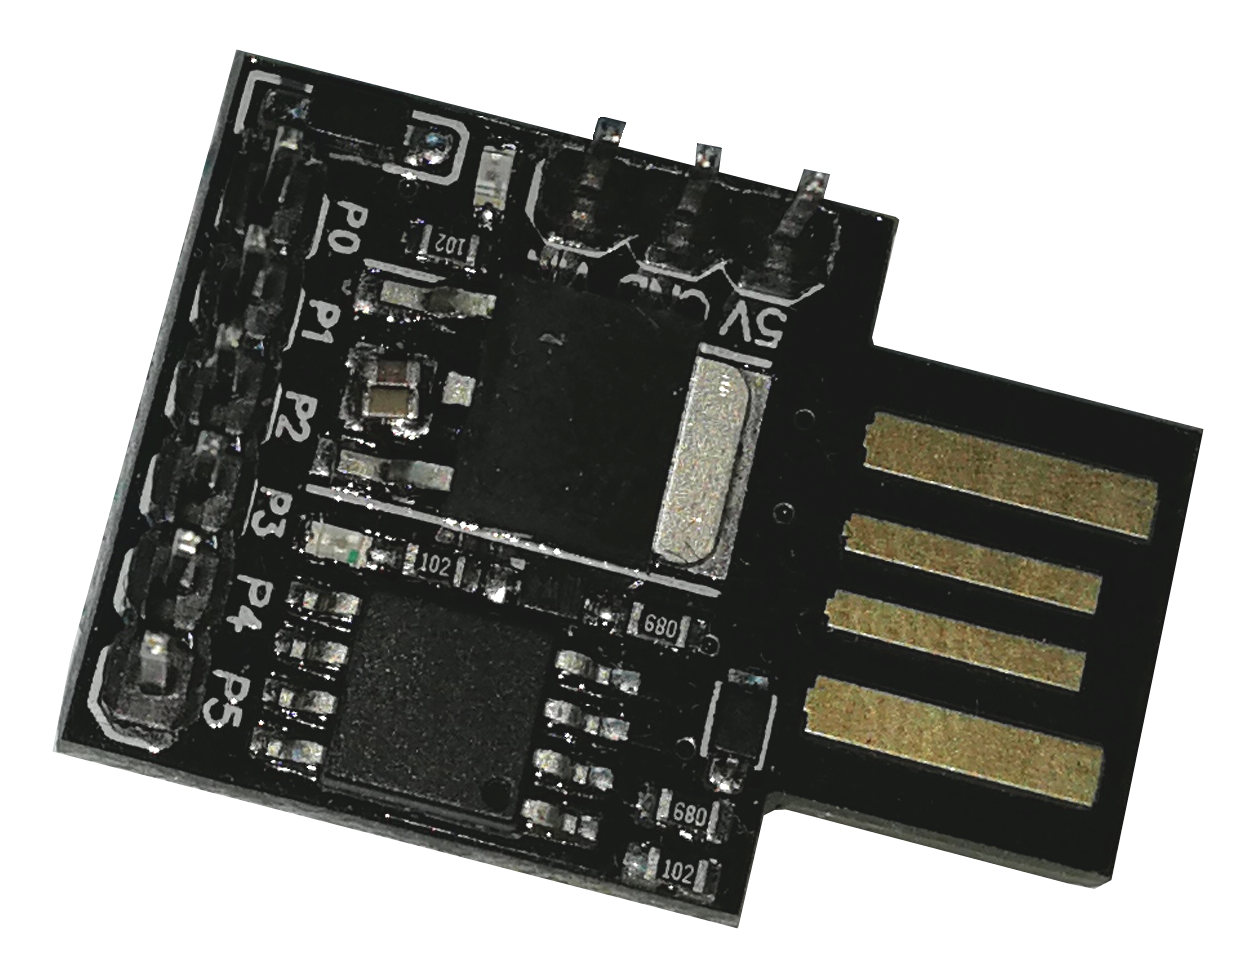
\includegraphics[width=4cm]{Images/digispark.png}
\caption{Digispark Rev. 3}
\label{fig:digispark}
\end{figure}

\subsubsection{Zweiter Entwurf}

		\begin{itemize}
			%\item Turtlebot beschreiben
			%\begin{itemize}
			%	\item Was ist der Turtlebot?
			%	\item Was kann er?
			%	\item Was wurde im Fachgebiet schon damit gemacht?
			%\end{itemize}
			
			\item Verwendete Soft- und Hardware
			\begin{itemize}
			\item Grafik vom 14.05. einbauen und beschreiben 
			\item Entscheidung für QT und RQT für die UI (Beschreiben)
				\item Roboterprogrammierung in C++
				\item Verwenden von QT oder Chromium für das Interface
				\item Verwenden von Arduino mit Taster als Sensor
				\item Optionale Idee: RFID-Leser mit Tags in Tassen oder Büchern
			\end{itemize}
			
		\end{itemize}
		
		
	\subsection{Umsetzung}
		Eric (Bis UI)\\
		Nach dem Kickoff-Meeting wurde vom Team beschlossen, sich einmal in der Woche im Labor des Fachgebiets zu treffen. Zu Beginn haben sich die Teammitglieder getrennt mit ... 
		\begin{itemize}
			\item Am Anfang Beschäftigung mit den Themen und Einarbeitung (Installation von Ubuntu und ROS)
			\item Besprechung mit dem Betreuer zu Konkretisierung des Auftrags

			\item Probleme durch Betriebssystem und Branches erwähnen
			\item Verwendung von Linux 16.04 als Betriebssystem
			\item Parallele Arbeit an Taster und UI
			\item Nachdem Laptop nicht funktioniert hat wurde auf den Rechner umgeschwenkt
		\end{itemize}
			\subsubsection{UI}
				Das User Interface (UI) wurde mit Hilfe der Software QTCreator erstellt. In dieser kann der Nutzer leicht Bedienelemente in ein Fenster hereinziehen und eine \glqq .ui\grqq-Datei wird erstellt. Für diese UI-Datei wurde danach in C++ eine Header- und Implementations-Datei mit den Namen \glqq rqt{\_}turtlebutler\grqq\ geschrieben.\\
				Das Interface wurde von Eric zu Hause erstellt und danach gemeinsam in den Treffen fertig gestellt. Die erste Version der UI enthielt noch Fehler im Programmcode, weswegen sie gebugfixt werden musste. Diese wurden auch zusammen behoben und die UI konnte zuerst am 9. Juli kompiliert werden.\\
				\begin{figure} [H]
					\centering
					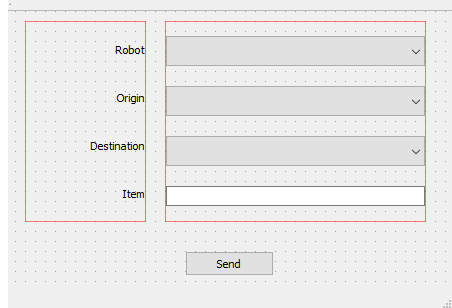
\includegraphics[height=6cm]{Images/Turtlebutler_Old.png}
					\caption{Alte Version des User-Interfaces in QTCreator}
					\label{fig:OldUI}
				\end{figure}
				Wie auf \cref{fig:OldUI} zu erkennen ist bestand die erste Version der UI einer Reihe an Dropdown-Menüs mit einem Knopf. In dem ersten Dropdown-Menü kann der Nutzer zwischen einem der drei Roboter des Fachgebiets, Leonardo, Donatello und Raphael, wählen. Die nächsten zwei Menüs dienen zur Auswahl des Abhol- und Zielpunktes. Zuletzt kann mit einer Texteingabe der gewünschte Gegenstand angegeben werden. Mit Hilfe des Drückens auf den Sendeknopf sollten diese Informationen nun in einer Nachricht verpackt werden, die an den gewählten Turtlebot geschickt wird.\\
				In der ersten Version wurde zunächst eine Konfigurationsdatei namens \glqq turtlebots.txt\grqq\ angelegt, in der Informationen zu den Turtlebots und festgelegten Punkten enthält. Die Daten in der Datei wurden mit Hilfe von Semikolons und Zeilenumbrüchen getrennt. Zuerst werden hier die Roboternamen mit ihren ROS-Topics gelesen und danach die Standortnamen mit deren X- und Y-Koordinaten.  Die gelesenen Daten wurden danach in die jeweiligen Dropdown-Menüs geschrieben. Der Nutzer kann hier nun die Namen von Turtlebots und Standorten sehen.\\
				Da die Nachrichten ohne ein passendes Behaviour-Skript auf der Roboter-Seite nicht funktionieren, wurde zuerst eine einfachere Nachricht verschickt. Hierfür wurde aus dem existierenden rviz-Plugin für den Turtlebot das ROS-Topic und der Nachrichtentyp entnommen. Zuerst soll nur eine \glqq Pose{\_}Stamped\grqq-Nachricht basierend auf dem gewählten Abholpunkt verschickt werden. Erhält der Turtlebot mit der bereits existierenden Konfiguration die Nachricht, so fährt er zu der gegebenen Position auf der Karte.\\
				Bei dem Erstellen der Konfigurationsdatei hat sich herausgestellt, dass jede Position von Hand durch Verschicken von Nachrichten mit dem rviz-Plugin aufgezeichnet werden muss. Auf Grund dessen wurde nach einem Gespräch mit dem Betreuer entschieden, eine bereits existierende Datei namens \glqq TopologicalModel.conf\grqq\ zu verwenden, in der sich eine Reihe aus Points of Interest (POIs) der Räume des Fachgebiets befinden.\\
				\textbf{ROBERT}: Umstellung auf existierende Kartendaten mit anderer Struktur (Karte entspricht nicht der Roboterkarte)\\
				\begin{figure} [H]
					\centering
					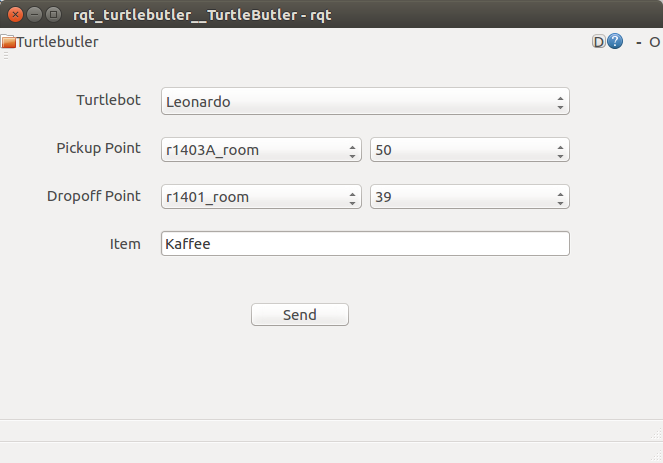
\includegraphics[height=8cm]{Images/Turtlebutler_Used.png}
					\caption{Aktuelle Version des User-Interfaces}
					\label{fig:NewUI}
				\end{figure}
				Auf Grund des Aufbaus der neuen POIs musste auch die UI verändert werden. Wie man an \cref{fig:NewUI} und \cref{fig:NewUIDropdown} sehen kann wurden die Dropdown-Menüs der Positionen in zwei Teile aufgeteilt. In dem linken Menü kann der Nutzer den Raum bestimmen und in dem Rechten die Position im Raum. Wählt der Nutzer einen Raum, so ändert sich dadurch die Liste an verfügbaren Positionen. Für das Verschicken der Nachricht ist hierbei nur die Position relevant, da diese mit den X- und Y-Koordinaten verknüpft ist. Da das Behaviour-Skript leider nicht fertig gestellt werden konnte, verschickt die neue UI weiterhin nur die Abholposition als \glqq Pose{\_}Stamped\grqq-Nachricht.
				\begin{figure} [H]
					\centering
					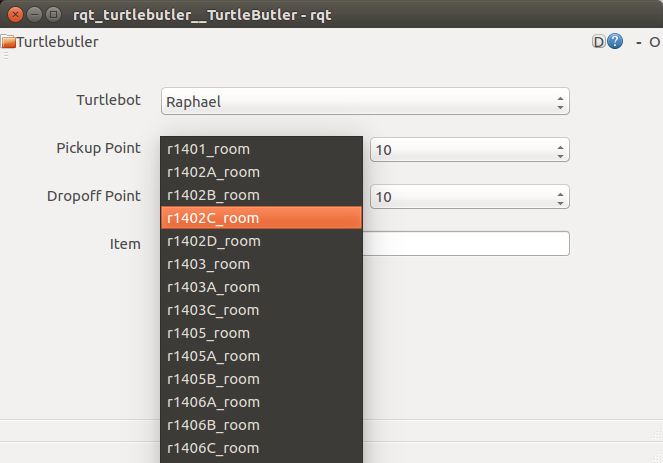
\includegraphics[height=5cm]{Images/Turtlebutler_Rooms.png}
					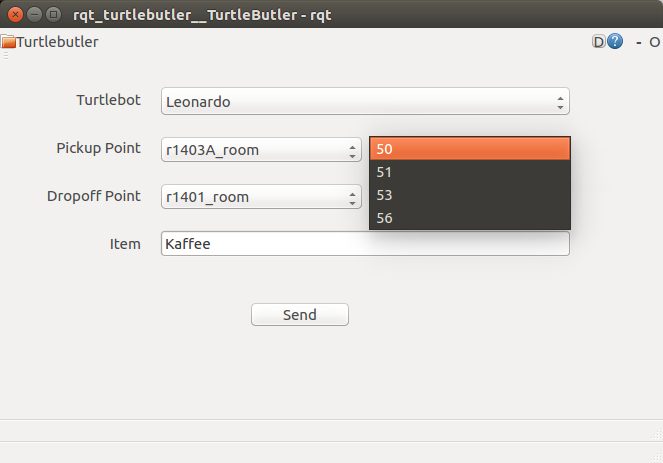
\includegraphics[height=5cm]{Images/Turtlebutler_Positions.png}
					\caption{Dropdown-Menüs des neuen User-Interfaces}
					\label{fig:NewUIDropdown}
				\end{figure}
%			\begin{itemize}
%				\item Verwenden von QTCreator zum Erstellen des UI-Fensters
%				\item Schreiben des Codes mit C++ und ROS (RQT)
%				\item Erstellen der UI zu Hause
%				\item Bugfixen auf dem Rechner als Team
%				\item Nachrichtenart vom rviz Plugin entnommen (Pose{\_}Stamped)
%				\item Erste Version zeigen (Bild) und beschreiben
%				\item Erste Version der Datenstruktur beschreiben
%				\item Fehler in der UI-Entwicklung beschreiben und Verbesserungen sagen
%				\item Error Handling bei schlechter Config Datei
%				\item Umstellung auf existierende Kartendaten mit anderer Struktur (Karte entspricht nicht der Roboterkarte) (Robert)
%				\item Verbesserung der UI mit den neuen Punkten (Zweite Version zeigen)
%			\end{itemize}
			
			\subsubsection{Taster}
			Dennis\\
			\begin{itemize}
				\item Rosserial Arduino zur Umwandlung in Nachrichten
				\item Entscheidung für Arduino
				\item Schreiben des Codes und Bauen des Tasters
				\item Einbauen des Tasters in das Weltmodell (Philipp)
				\item Verbesserung des Tasters mit Korb aus Haribo
			\end{itemize}
	
	\subsection{Ausblick}
	Eric \\
	\begin{itemize}
		\item Auftrag ist nicht ganz fertig geworden
		\item Schreiben eines Behaviours, das den Taster verwendet
		\item Verwenden von anderen Nachrichtentypen zum Senden
		\item Anpassen der Kartendaten mit Roboter-Infos
		\item Roboter kann per Text to Speech den gesuchten Gegenstand sagen
		\item Verwendung von RFID zur Erkennung der Gegenstände
	\end{itemize}
	\newpage
	\section{Teamarbeit}
	
	\subsection{Teamrollen}
		In dem Kickoff-Meeting wurden zwei Aufteilungen von Teamrollen vorgestellt: Teamrollen nach Basadur und nach Belbin.
		\begin{figure} [H]
			\centering
			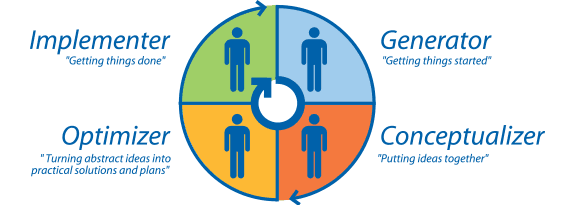
\includegraphics[height=4.5cm]{Images/Basadur.png}
			\caption{Teamrollen nach Basadur}
			\label{fig:Basadur}
		\end{figure}
		Auf \cref{fig:Basadur} sind die Teamrollen nach Basadur zu sehen. Diese wurden in Generator, Conceptualizer, Optimizer und Implementer aufgeteilt. Der \textbf{Generator} ist derjenige, der Dinge ins Rollen bringt und viele Ideen zur Problemlösung sucht. Hierbei ist es schwer, ihn auf eine Idee festzunageln. Der \textbf{Conceptualizer} nimmt die Ideen vom Generator und versucht diese zusammen mit eigenen zu verwenden, um nach Lösungen zu suchen. Er versucht dabei, das Problem vollständig zu begreifen. Der \textbf{Optimizer} nutzt die abstrakten Ideen von Generator und Conceptualizer zur Umsetzung. Meist fokussiert er sich auf ein Problem und vertraut auf seine eigenen Fähigkeiten bei der Suche nach Lösungen. Der \textbf{Implementer} probiert Dinge lieber praktisch aus und verwirft Theorien, die nicht zu dieser Praxis passen. Er ist enthusiastisch und kann gut mit Menschen arbeiten. Dadurch wirkt er manchmal ungeduldig und aufdringlich.\\
		\begin{figure} [H]
			\centering
			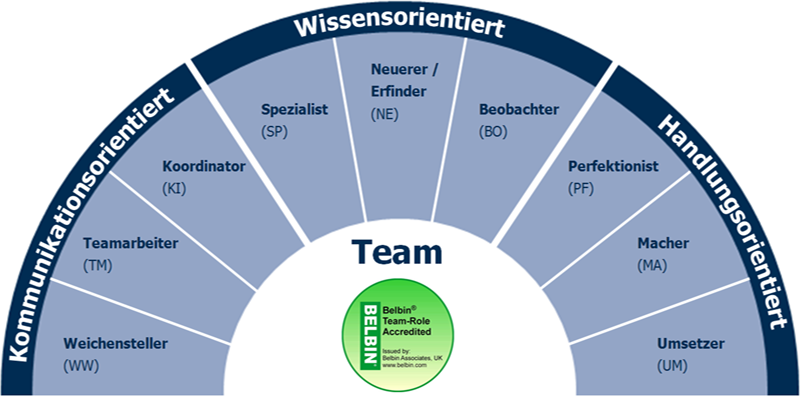
\includegraphics[height=6cm, width=12cm]{Images/Belbin.png}
			\caption{Persönlichkeiten im Team nach Belbin}
			\label{fig:Belbin}
		\end{figure}
		Auf \cref{fig:Belbin} kann man die Teampersönlichkeiten nach Belbin sehen, diese sind in drei Kategorien unterteilt, sodass ein Teammitglied meist mehr als einen Typ hat. Im Folgenden werden die Rollen mit jeweils einem Satz beschrieben.\\
		Der \textbf{Weichensteller} kommuniziert innerhalb und außerhalb des Teams.\\
		Der \textbf{Teamarbeiter} ist anpassungsfähig und arbeitet flexibel mit den anderen.\\
		Der \textbf{Koordinator} versucht, alle zum gemeinsamen Ziel zu bewegen.\\
		Der \textbf{Spezialist} hat besondere Fähigkeiten, die er zum Lösen der Aufgabe gebrauchen kann.\\
		Der \textbf{Erfinder} findet Ideen, die als Grundlage für die Arbeit verwendet werden können.\\
		Der \textbf{Beobachter} überdenkt Aufgaben kritisch und sucht nach Lösungen.\\
		Der \textbf{Perfektionist} achtet auf Details und verfolgt Dinge bis zum Ende.\\
		Der \textbf{Macher} arbeitet hochmotiviert und möchte etwas erreichen.\\
		Der \textbf{Umsetzer} hat einen Sinn fürs Praktische und geht systematisch vor.\\
		
		In den folgenden Abschnitten haben sich die Teammitglieder selber und gegenseitig ein den Teamrollen nach Basadur und Belbin eingeschätzt.
		\subsubsection{Dennis}
		Basadur: \\
		Belbin: 
		\subsubsection{Robert}
		Basadur: \\
		Belbin: 
		\subsubsection{Philipp}
		Basadur: \\
		Belbin: 
		\subsubsection{Eric}
		In den Teamrollen nach Basadur schätzt sich Eric als \textbf{Conceptualizer} und \textbf{Optimizer} ein. Als Conceptualizer hat er zu Beginn des Projektes Ideen gesammelt und das Problem in Unterprobleme aufgeteilte. Er sammelte die Ideen und versuchte diese umzusetzen und zu überdenken. Beim Umsetzen der Ideen und Problemlösen hat er sich mit den anderen Teammitgliedern zusammengefunden und gemeinsam nach Lösungswegen und Lösungen zu suchen. Als Generator schätzt sich Eric weniger ein, da er sich meist auf eine Idee festlegt und selber selten zu Ideen kommt. Zusätzlich denkt er von sich nicht als Implementer, da er meist eher theoretisch über Ideen nachdenkt und Theorien aufstellt. Trotzdem kann er wie ein Implementer gut mit Menschen arbeiten.\\
		Bei den Teamtypen nach Belbin sieht sich Eric als \textbf{Weichensteller} und \textbf{Koordinator}. Im Laufe der Teamarbeit hat er sich als Teamleiter etabliert, indem er die Arbeit bei den wöchentlichen Team-Treffen protokolliert hat. Dazu koordinierte er die Teammitglieder und versuchte bei Besprechungen jeden mit einzubeziehen. War ein Teammitglied nicht anwesend bei dem Treffen, so wurde diese Person von Eric entweder direkt danach durch die WhatsApp-Chatgruppe oder zum nachfolgenden Treffen informiert, was sie verpasst hatte. Zum Teil lässt sich Eric noch als \textbf{Spezialist} einschätzen, da er vor dem Projekt bereits mit ROS, Arduino und UIs gearbeitet hat.\\
		
\subsubsection{Vorwissen der Teammitglieder}
			\begin{itemize}
				\item Robert: Erfahrungen in Linux
				\item Eric: Erfahrungen in UI-Programmierung
				\item Dennis: Erfahrungen mit Tastern und Hardware
			\end{itemize}
	\subsection{Teamphasen}
		Dennis\\
		Grafik der Phasen einbauen.
	\subsubsection{Forming}
		Bis wohin wurde nix geschafft? Teamfindung.
	\subsubsection{Storming}
		Aushilfe vom Betreuer. Sachen kompilieren und funktionieren.
	\subsubsection{Norming}
		Kickoff-Meeting. 
	\subsubsection{Performing}
		Abschluss. Dokumentation.
	\subsection{Probleme und Lösungen}
		Philipp\\
		Komplikationen mit dem Turtlebot
		\begin{itemize}
			\item Falsche Branches (Mit Betreuer gelöst)
			\item Akku kaputt (Tausch des Akkus durch Betreuer)
			\item Kommunikation nicht möglich (Deaktivieren eines Netzwerks)
			\item Kartendaten sind nicht akkurat auf den Turtlebot zugeschnitten
		\end{itemize}
		Am Protokol orientieren.
	\section{Fazit}
		(Gemeinsam, jeder ein Absatz?)
		Wie hat die Arbeit im Team funktioniert? Anwendung der Workshop-Sachen auf reale Teamarbeit.
		
	\newpage
	\section{Quellen}
		\begin{itemize}
			\item ROS - \href{http://www.ros.org/}{http://www.ros.org/}
			\item Turtlebot - \href{https://www.turtlebot.com/}{https://www.turtlebot.com/}
			\item QT und QTCreator - \href{https://www.qt.io/}{https://www.qt.io/}
			\item RQT (ROS-QT) - \href{http://wiki.ros.org/rqt}{http://wiki.ros.org/rqt}
		\end{itemize}
\end{document}